\subsection{Model Parameter Estimates in the Limit of Large Data Sets} \label{sec:largedata}

%====================================================================

%FIGURE: Triangle plot, shape of likelihood, multi-variate Gaussian

\begin{figure*}[!htbp]
\centering
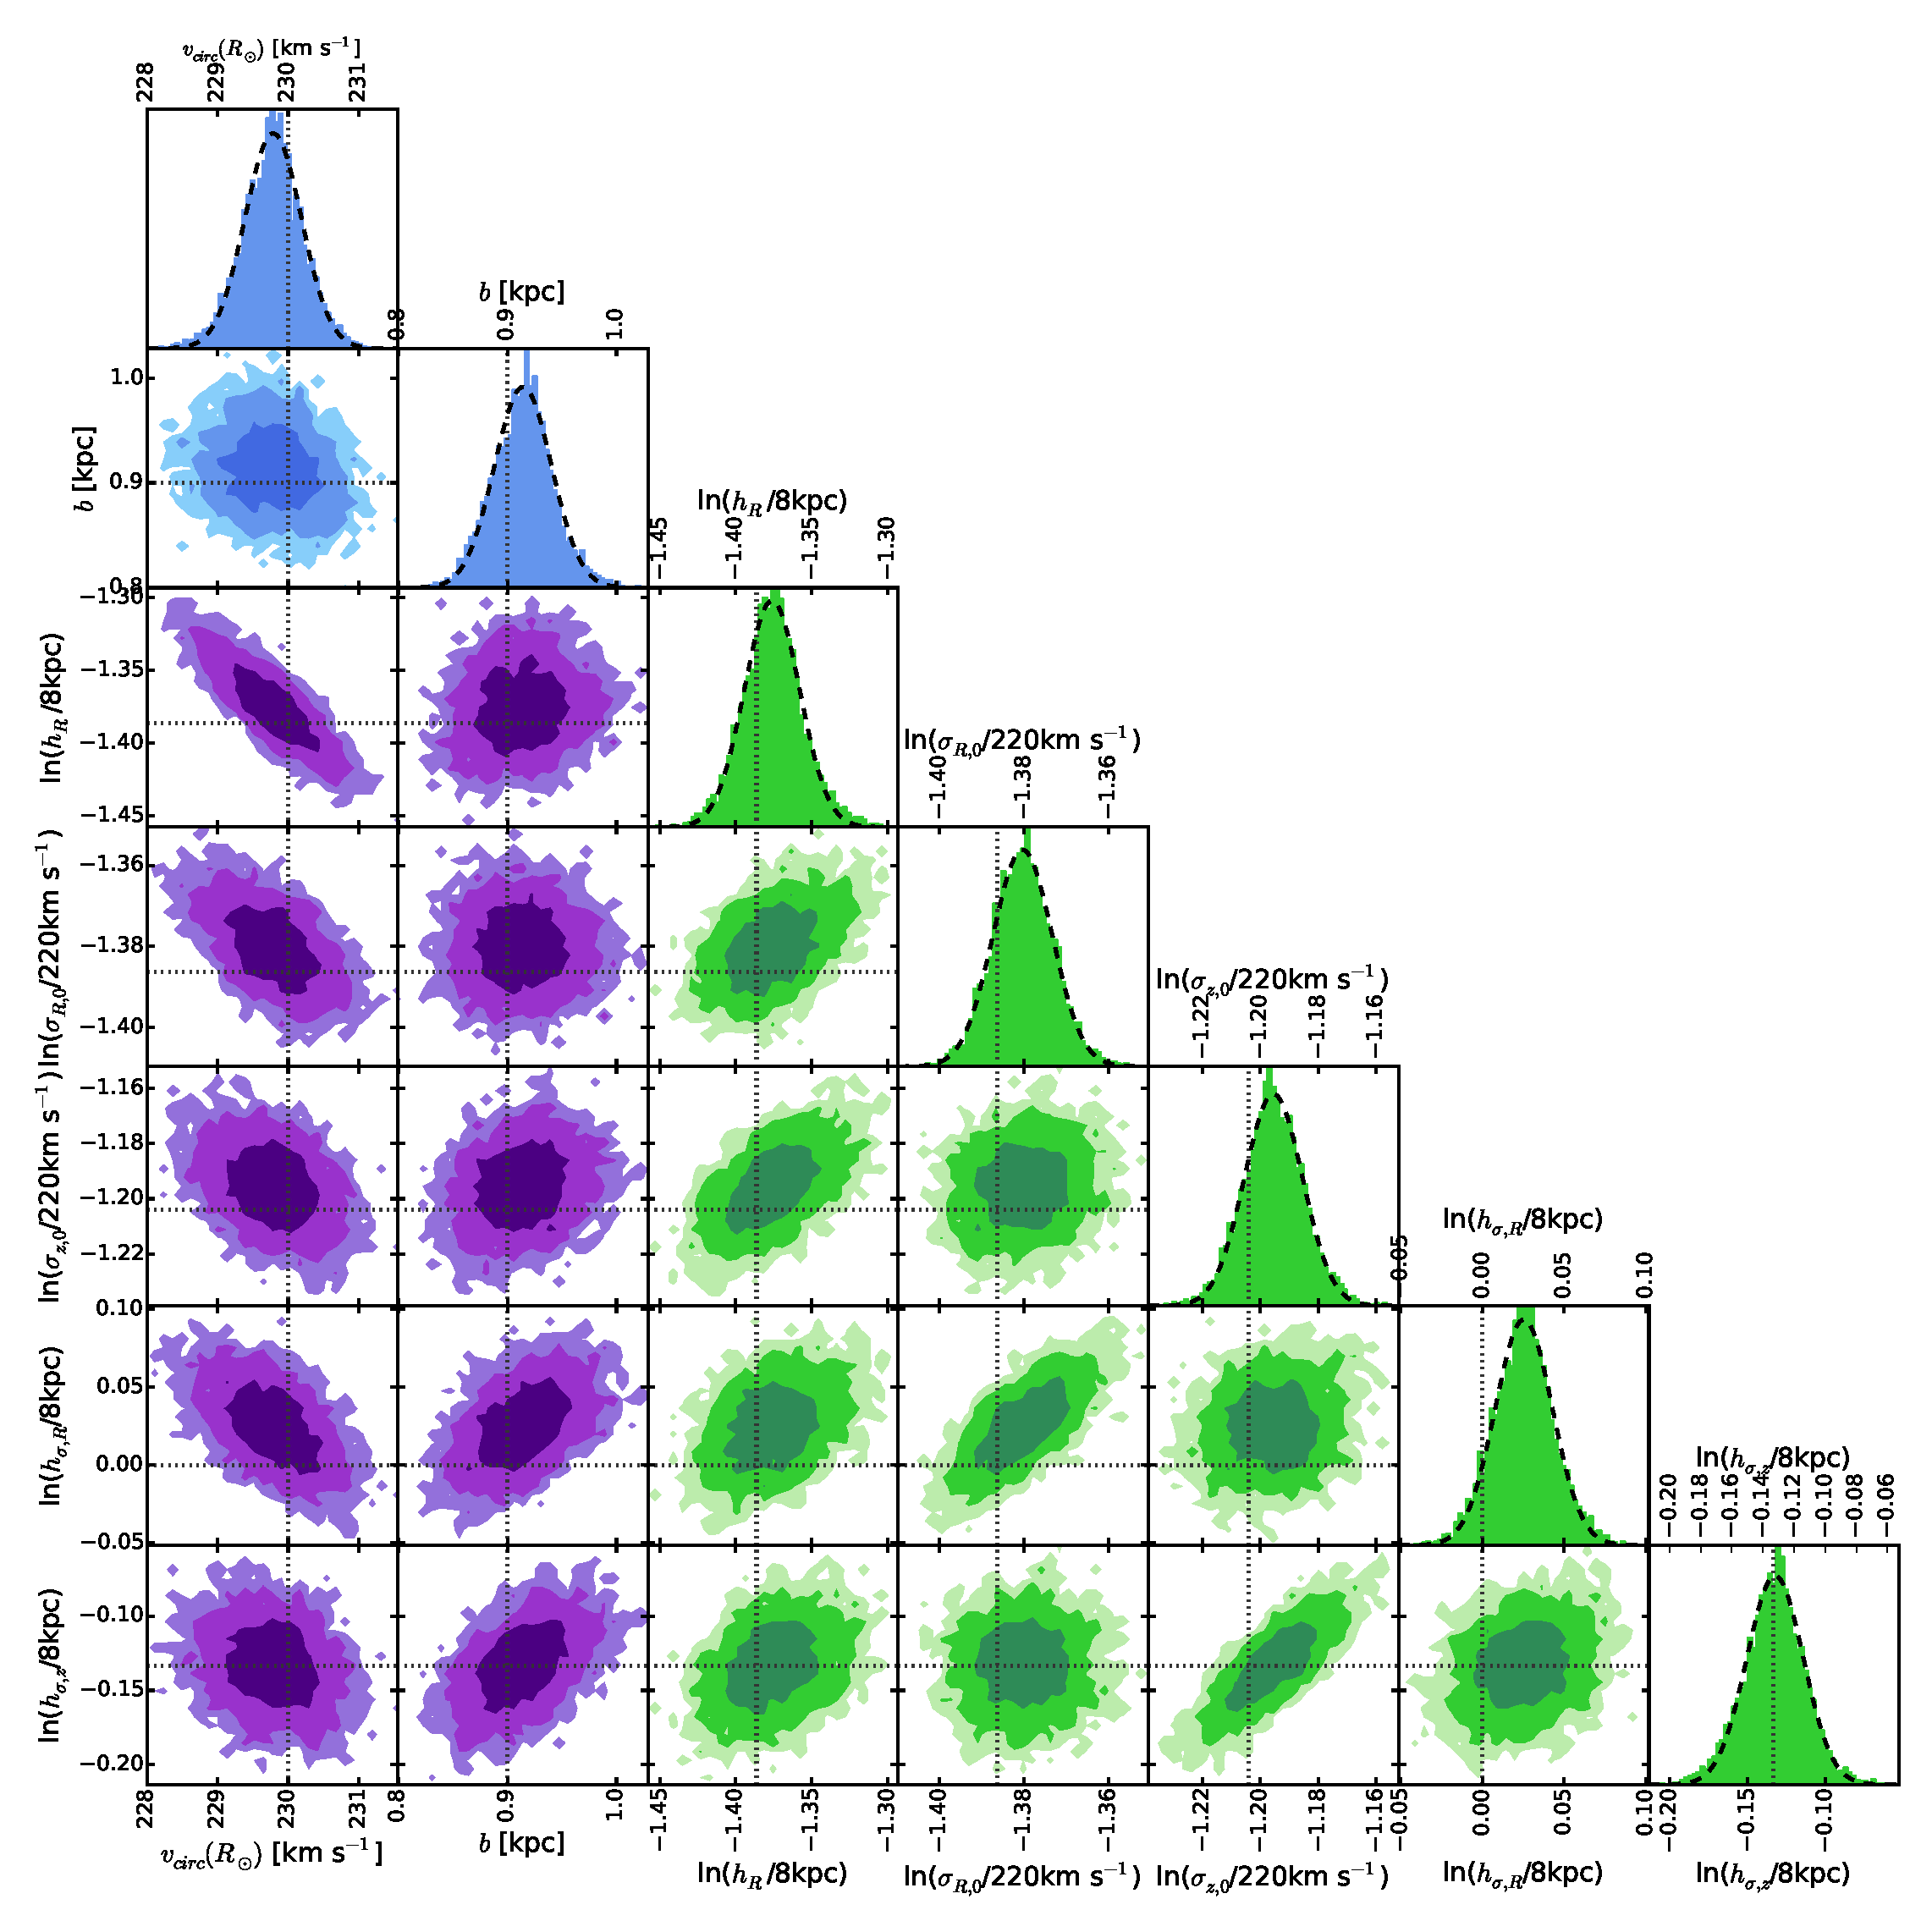
\includegraphics[width=0.7\textwidth]{figs/isoSphFlex_short_hot_2kpc_triangle_MCMC.eps}
\caption{The \pdf{} (proportional to the likelihood in Equation \ref{eq:prob}) in the parameter space $\pmodel{} = \{p_\Phi,p_\text{DF}\}$ for one example mock data set created according to Test \ref{test:isoSphFlex} in Table \ref{tbl:tests}. Blue indicates the \pdf{} for the potential parameters, green the qDF parameters. The true parameters are marked by dotted lines. The dark, medium and bright contours in the 2D distributions represent 1, 2 and 3 sigma confidence regions \HW{[TO DO: HW: "likelihood vs. pdf - This is where this matters: is this a confidence on the data or on the parameters?" Don't understand, what he means...]}, respectively. The parameters are weakly to moderately covariant, but their level of covariance depends on the actual choice of the mock data's \pmodel{}. The \pdf{} here was sampled using MCMC. The dashed lines in the 1D distributions are Gaussian fits to the histogram of MCMC samples. This demonstrates very well that for such a large number of stars, the \pdf{} approaches the shape of a multi-variate Gaussian, as expected from the central limit theorem \Jo{[TO DO: Jo wrote, that he is not sure if the central limit theorem is directly relevant here]}.}
\label{fig:isoSphFlex_triangleplot}
\end{figure*}

%====================================================================

%FIGURE: width of likelihood propto 1/sqrt(N)

\begin{figure}[!htbp]
\plotone{figs/sqrtNiso_Stddev_Vs_N.eps}
\caption{The width of the \pdf{} (see Equation \ref{eq:prob}) for two fit parameters found from analyses of 132 mock data sets vs. the number of stars in each data set. (The mock data was created according to the model parameters given in Test \ref{test:sqrtNiso} in Table \ref{tbl:tests}.) The relative standard error (SE) was found from a Gaussian fit to the marginalized \pdf{} for each model parameter. As can be seen, for large data samples the width of the \pdf{} scales with $1/\sqrt{N_{*}}$ as predicted by the central limit theorem.} 
\label{fig:sqrtNiso}
\end{figure}

%====================================================================


%FIGURE: central limit theorem is satisfied

\begin{figure}[!htbp]
\centering
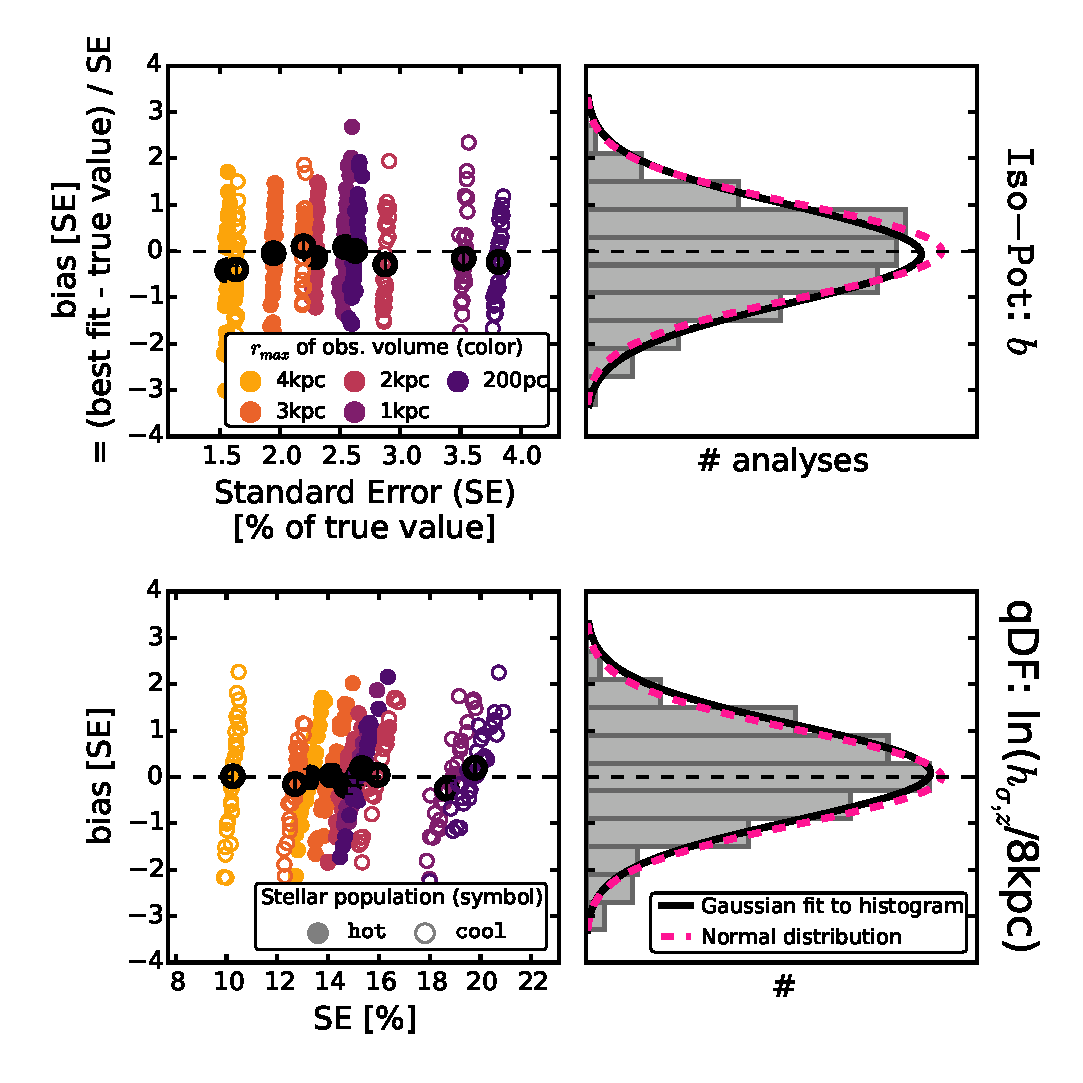
\includegraphics[width=\columnwidth]{figs/isoSph_CLT_2.eps}
\caption{(Un-)bias of the parameter estimates: According to the central limit theorem the the best fit values for a large number of data sets, each containing a large number of stars, will follow the Normal distribution. To test this, we create 320 mock data sets, which come from two different stellar populations and five spherical observation volumes (see legends). (All model parameters are summarized in Table \ref{tbl:tests} as Test \ref{test:isoSph_CLT}.) Bias and relative standard error (SE) are derived from the marginalized \pdf{} for one potential parameter (isochrone scale length $b$ in first row) and one qDF parameter ($h_{\sigma,z}$ in second row). The second column displays a histogram of the 320 offsets. As it closely follows a Normal distribution, our modelling method is therefore well-behaved and unbiased. The black dots show the mean offset and SE for the 32 analyses belonging to one model. \Wilma{ [TO DO: $r_\text{max}$ instead of radius in legend] [TO DO: Leerzeichen fehlt in y-achsenbeschriftung] [TO DO: no kpc at b, and / 8kpc at hsz]}}
\label{fig:isoSph_CLT}
\end{figure}

%====================================================================


The individual \MAP{}s in BR13 contained typically between 100 and 800 objects, so that each \MAP{} implied a quite broad \pdf{} for the model parameters $\pmodel{}$. Here we explore what happens in the limit of much larger samples, say $N_{*} = 20,000$ objects. As outlined in \S\ref{sec:likelihood} the immediate consequence of larger samples is given by the likelihood normalization requirement, $\log(1+\delta M_\text{tot})\le 1/N_{*}$, (see Equation \ref{eq:loglikelihood_relerr})), which is the modelling aspect that drives the computing time. This issues aside, we would, however, expect that in the limit of large data sets with vanishing measurement errors the \pdf{}s of the \pmodel{} become Gaussian, with a \pdf{} width that scales as $1/\sqrt{N_{*}}$. Further, we must verify that any bias in the \pdf{} expectation value is considerably less than the error, even for quite large samples.

Using sets of mock data, created according to \S\ref{sec:mockdata} and a fiducial model for \pmodel{} (see Table \ref{tbl:tests}, Tests \ref{test:sqrtNiso}, \ref{test:isoSph_CLT}, and \ref{test:isoSphFlex}), we verified that \RM{} satisfies all these conditions and expectations: Figure \ref{fig:isoSphFlex_triangleplot} illustrates the joint \pdf{}s of all \pmodel{}. The \pdf{} is a multivariate Gaussian that projects into Gaussians when considering the marginalized \pdf{} for all the individual \pmodel{}. Figure \ref{fig:sqrtNiso} then demonstrates that the \pdf{} width indeed scales as $1/\sqrt{N_{*}}$. Figure \ref{fig:isoSph_CLT} illustrates even more that \RM{} satisfies the central limit theorem. The average parameter estimates from many mock samples with identical underlying \pmodel{} are very close to the input \pmodel{}, and the distribution of the actual parameter estimates are a Gaussian around it. 

